
\documentclass[11pt,a4paper]{article}
\usepackage[utf8]{inputenc}
\usepackage[T1]{fontenc}
\usepackage[spanish,es-nodecimaldot]{babel}
\usepackage[a4paper,left=1.7cm,right=1.7cm,top=20mm,bottom=20mm]{geometry}
\usepackage{amsmath,amssymb,amsfonts,mathtools,bm}
\usepackage{braket}
\usepackage{graphicx}
\usepackage{float}
\usepackage{booktabs}
\usepackage{enumitem}
\usepackage{xcolor}
\usepackage{lmodern,microtype}
\usepackage{fancyhdr}
\usepackage{titlesec}
\usepackage[colorlinks=true,linkcolor=black,urlcolor=black,citecolor=black]{hyperref}
\numberwithin{equation}{section}
\renewcommand{\boxed}[1]{#1}
\setlength{\parindent}{0pt}
\setlength{\parskip}{5pt}
\newcommand{\dd}{\,\mathrm d}
\newcommand{\ii}{\mathrm i}
\newcommand{\e}{\mathrm e}
\newcommand{\hb}{\hbar}
\newcommand{\R}{\mathbb R}
\newcommand{\C}{\mathbb C}
\newcommand{\id}{\mathbb I}

\pagestyle{fancy}
\setlength{\headheight}{14pt}
\fancyhf{}
\fancyhead[L]{\textit{Tarea 13}}
\fancyhead[R]{Mecánica Cuántica I}
\begin{document}
\begin{titlepage}
\centering
\vspace*{1.8cm}

\includegraphics[width=.22\textwidth]{UdeC_escudo.png}
\vspace{1.1cm}
{\Huge\bfseries Tarea 13\par}
\vspace{.4cm}
{\Huge\bfseries Mecánica Cuántica I\par}
\vspace{1.5cm}
{\Large José Ignacio Rosas Sepúlveda\par}
\vspace{.8cm}
{\Large Solución\par}
\vfill
\thispagestyle{empty}
\end{titlepage}
\tableofcontents
\newpage
\section*{Enunciado}
\addcontentsline{toc}{section}{Enunciado}
El espacio de Hilbert de una partícula de spin $1/2$ es bidimensional. Sean
\begin{equation}
S_x=\frac{\hbar}{2}\sigma_x,\qquad
S_y=\frac{\hbar}{2}\sigma_y,\qquad
S_z=\frac{\hbar}{2}\sigma_z.
\end{equation}
Inicialmente $\ket{\psi(0)}=\ket\downarrow$. La partícula interactúa con el campo
\begin{equation}
\mathbf B=\left(\frac{B}{\sqrt2},0,\frac{B}{\sqrt2}\right),
\end{equation}
de modo que
\begin{equation}
H=-\gamma\mathbf S\cdot\mathbf B
=-\frac{\gamma\hbar B}{2\sqrt2}(\sigma_x+\sigma_z).
\end{equation}
\begin{enumerate}[label=\arabic*.]
\item Encuentre los valores y estados propios de $H$.
\item Encuentre $U(t)$.
\item Encuentre $\ket{\psi(t)}$.
\item Si se mide $H$, indique resultados y probabilidades.
\item Represente $\ket{\psi(t)}$ en la base propia de $S_z$.
\item Encuentre $\langle S_x(t)\rangle$, $\langle S_y(t)\rangle$ y $\langle S_z(t)\rangle$.
\item Grafique esos promedios, normalizados por $\hbar/2$, como funciones de $\tau=\gamma Bt$.
\item Encuentre $\Delta S_x(t)$, $\Delta S_y(t)$ y $\Delta S_z(t)$.
\item Grafique esas desviaciones, normalizadas por $\hbar/2$, como funciones de $\tau$.
\item Si se mide $S_z$, indique resultados y probabilidades.
\item Represente $\ket{\psi(t)}$ en la base propia de $S_x$.
\item Si se mide $S_x$, indique resultados y probabilidades.
\end{enumerate}


\section{Problema 1}
El campo es
\begin{equation}
\bm B=\frac{B}{\sqrt2}(1,0,1),
\end{equation}
y
\begin{equation}
H=-\gamma\bm S\cdot\bm B
=-\frac{\hb\Omega}{2}\,\hat n\cdot\bm\sigma,
\qquad \Omega=\gamma B,
\qquad \hat n=\frac1{\sqrt2}(1,0,1).
\end{equation}
La dirección $\hat n$ tiene $\theta=\pi/4$, $\varphi=0$. Los estados propios de $\hat n\cdot\bm\sigma$ son
\begin{align}
\ket{n,+}&=\cos\frac\pi8\ket\uparrow+\sin\frac\pi8\ket\downarrow,\\
\ket{n,-}&=-\sin\frac\pi8\ket\uparrow+\cos\frac\pi8\ket\downarrow.
\end{align}
Por tanto,
\begin{equation}
\boxed{E_+=-\frac{\hb\Omega}{2},\qquad E_-=+\frac{\hb\Omega}{2}.}
\end{equation}

\section{Problema 2}
Como $(\hat n\cdot\bm\sigma)^2=\id$,
\begin{equation}
\boxed{U(t)=\cos\frac\tau2\,\id+\ii\sin\frac\tau2\,\frac{\sigma_x+\sigma_z}{\sqrt2},\qquad \tau=\Omega t.}
\end{equation}
Aplicándolo a $\ket{\psi(0)}=\ket\downarrow$,
\begin{equation}
\boxed{\ket{\psi(t)}=
\frac{\ii}{\sqrt2}\sin\frac\tau2\ket\uparrow+
\left(\cos\frac\tau2-\frac{\ii}{\sqrt2}\sin\frac\tau2\right)\ket\downarrow.}
\end{equation}

\subsection{Medición de energía}
Como las probabilidades en la base propia de $H$ son constantes,
\begin{align}
P(E_+)&=|\braket{n,+|\downarrow}|^2=\sin^2\frac\pi8
=\frac12\left(1-\frac1{\sqrt2}\right),\\
P(E_-)&=\cos^2\frac\pi8
=\frac12\left(1+\frac1{\sqrt2}\right).
\end{align}

\section{Problema 3}
El vector de Bloch del estado es
\begin{equation}
\bm r(t)=\left(\frac{\cos\tau-1}{2},\,-\frac{\sin\tau}{\sqrt2},\,-\frac{1+\cos\tau}{2}\right).
\end{equation}
Por ello,
\begin{equation}
\boxed{\langle S_i\rangle=\frac\hb2r_i,\qquad
\Delta S_i=\frac\hb2\sqrt{1-r_i^2}.}
\end{equation}
\begin{figure}[H]\centering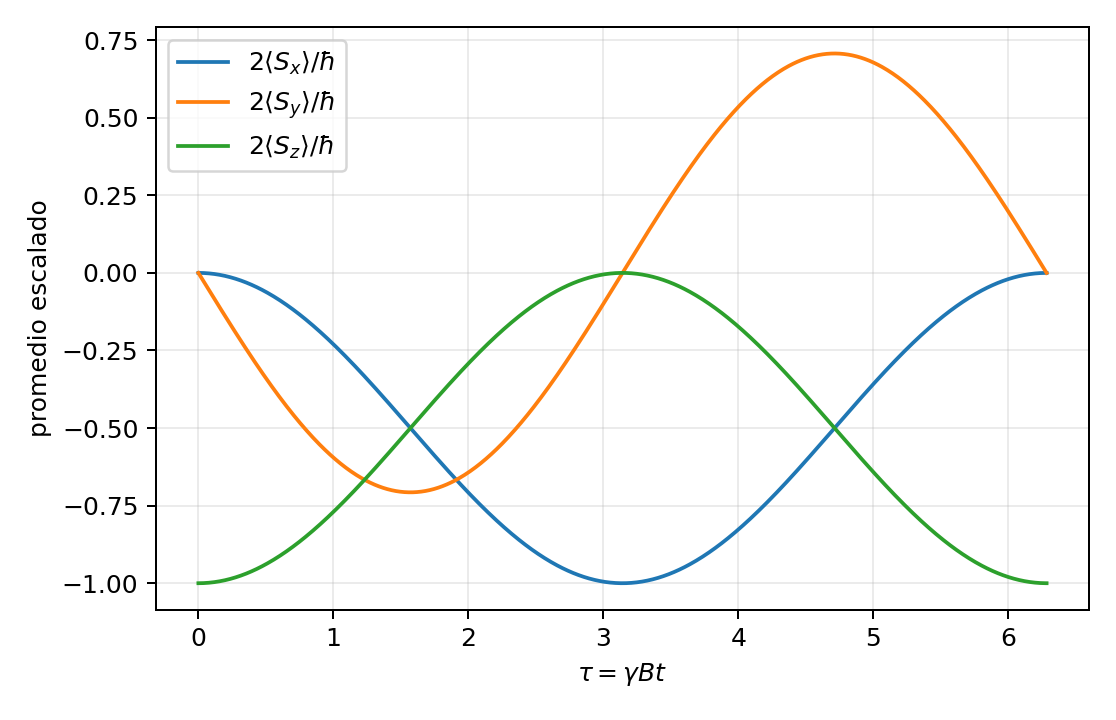
\includegraphics[width=.70\textwidth]{figures/spin_promedios.png}\caption{Promedios de las tres componentes.}\end{figure}
\begin{figure}[H]\centering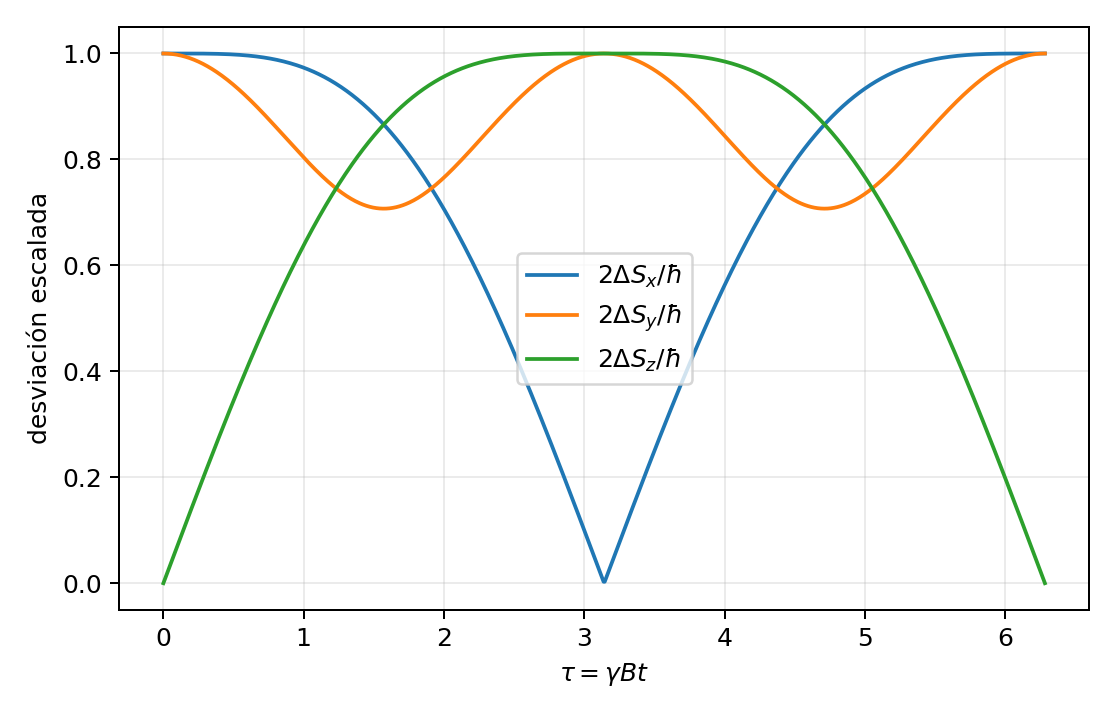
\includegraphics[width=.70\textwidth]{figures/spin_desviaciones.png}\caption{Desviaciones estándar de las tres componentes.}\end{figure}

\section{Problema 4}
Para $S_z$,
\begin{equation}
P(\uparrow_z)=\frac{1+r_z}{2}=\frac{1-\cos\tau}{4},
\qquad
P(\downarrow_z)=\frac{3+\cos\tau}{4}.
\end{equation}
Para $S_x$,
\begin{equation}
P(+x)=\frac{1+r_x}{2}=\frac{1+\cos\tau}{4},
\qquad
P(-x)=\frac{3-\cos\tau}{4}.
\end{equation}
La representación en la base $S_x$ se obtiene de
\begin{equation}
\ket\uparrow=\frac{\ket{+x}+\ket{-x}}{\sqrt2},\qquad
\ket\downarrow=\frac{\ket{+x}-\ket{-x}}{\sqrt2},
\end{equation}
sustituyendo las amplitudes anteriores.


\end{document}
